% meta.concepts: beam shear and bending moment diagram
% meta.tags: realistic
% acknowledge: Peter Seiler & Luke Melander graciously shared Spring 2019 course material
% source: P. Seiler AEM2011 Spring 2014 Exam 2 (modified)

\noindent Last weekend was not warm but Professor Seiler was determined to go for a swim. The
diving board at his local pool is shown below (left figure). The board is pinned at A and supported by a rolling
joint at B, as shown in the simplified diagram (right figure). Assume:
\begin{itemize}
  \item The board is rigid and has a total length of $4.3$ $m$.
  \item He stands on the last $0.3$ $m$ of the board and his weight is distributed as $w(x) = 25000$ $N/m$.
  \item The reaction forces at $A$ and $B$ are $A = -8062.5N \bf j$ and $B = 15562.5N \bf j$.
\end{itemize}

\noindent Sketch the shear force $V(x)$ and bending moment $M(x)$ diagram for the diving board (i.e. along $x$).

\begin{figure*}[ht!]
  \centering
  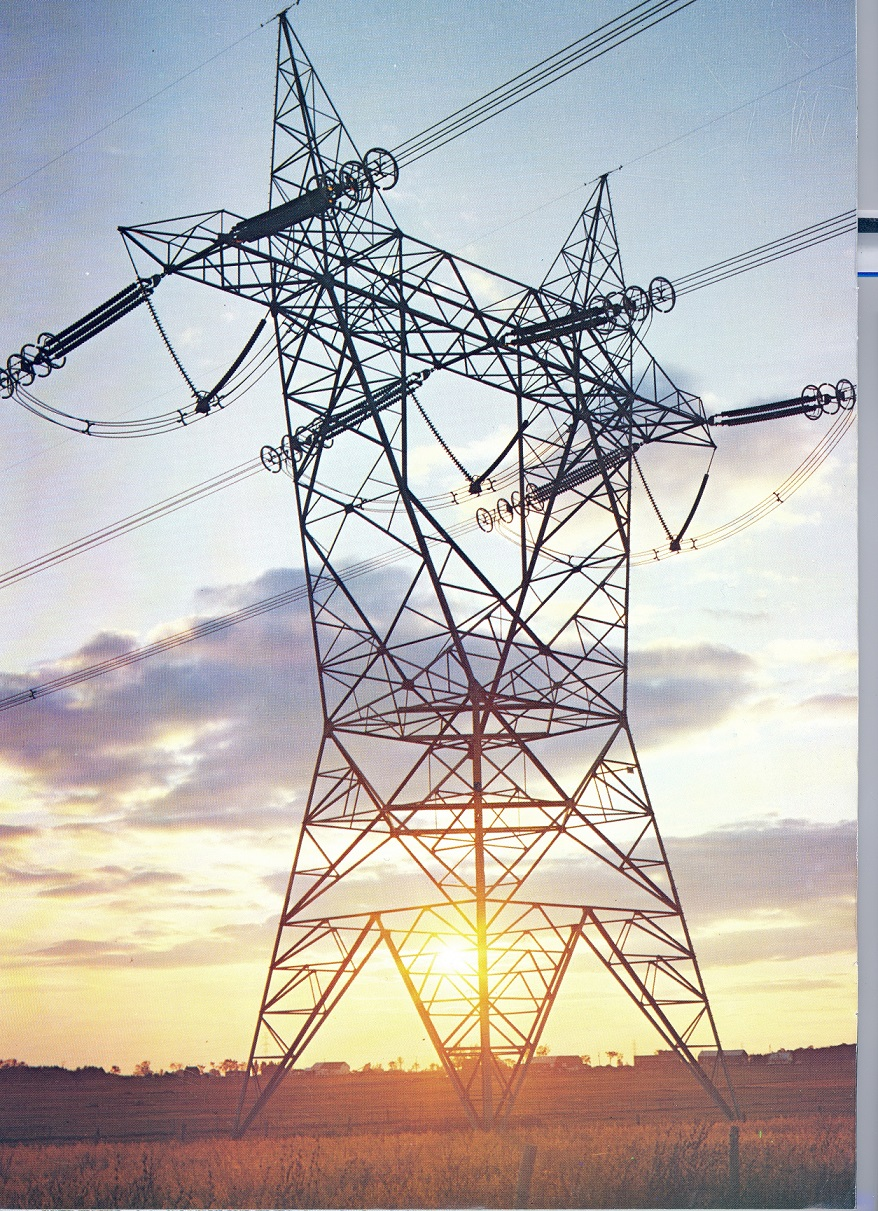
\includegraphics[width=0.4\textwidth,
	           height=0.3\textheight,
		   keepaspectratio]{figa.png}
  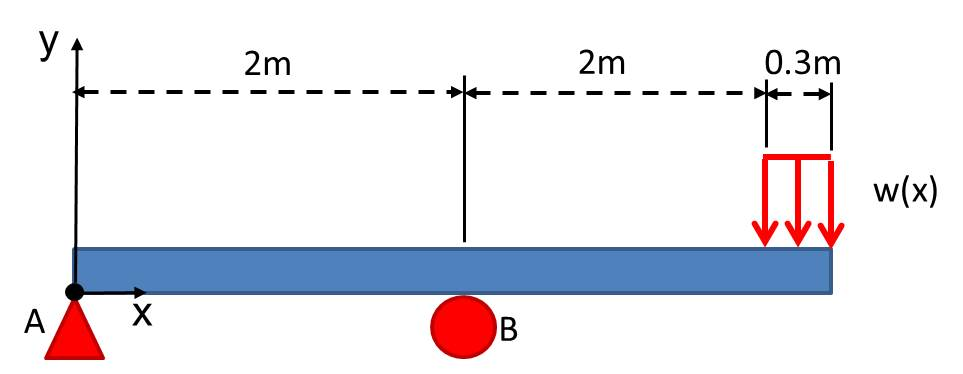
\includegraphics[width=0.4\textwidth,
	           height=0.3\textheight,
		   keepaspectratio]{figb.png}
\end{figure*}

